\documentclass[a4paper,14pt]{extarticle}
\usepackage[T2A]{fontenc}
\usepackage[utf8]{inputenc}
\usepackage[english,russian]{babel}
\usepackage{amsmath,amsfonts,amsthm, mathtools}
\usepackage{amssymb}
\usepackage{icomma}
\usepackage{graphicx}
\usepackage{wrapfig}
\RequirePackage{longtable}
\usepackage{soulutf8} 
\usepackage{geometry}
\geometry{top=20mm}
\geometry{bottom=20mm}
\geometry{left=20mm}
\geometry{right=20mm}


\usepackage{cmap}					
\usepackage{mathtext} 				
			
		

\usepackage{multirow}
\usepackage{graphicx}
\usepackage{wrapfig}
\usepackage{tabularx}
\usepackage{float}
\usepackage{hyperref}
\hypersetup{colorlinks=true,urlcolor=blue}
\usepackage[rgb]{xcolor}
\usepackage{amsmath,amsfonts,amssymb,amsthm,mathtools} 
\usepackage{icomma} 
\usepackage{euscript}
\usepackage{mathrsfs}
\usepackage{enumerate}
\usepackage{caption}
\usepackage{enumerate}
\mathtoolsset{showonlyrefs=true}

\usepackage{caption}
\usepackage{subcaption}

\usepackage[europeanresistors, americaninductors]{circuitikz}
\DeclareMathOperator{\sgn}{\mathop{sgn}}
\newcommand*{\hm}[1]{#1\nobreak\discretionary{}
	{\hbox{$\mathsurround=0pt #1$}}{}}

\begin{document}
	
	\begin{center}
		\textit{Федеральное государственное автономное образовательное\\ учреждение высшего образования }
		
		\vspace{0.5ex}
		
		\textbf{«Московский физико-технический институт\\ (национальный исследовательский университет)»}
	\end{center}
	
	\vspace{10ex}
	
	
	\begin{center}
		\vspace{13ex}
		
		\textbf{Лабораторная работа №1.4.1}
		
		\vspace{1ex}
		
		по курсу общей физики
		
		на тему:
		
		\textbf{\textit{<<Физический маятник>>}}
		
		\vspace{30ex}
		
		\begin{flushright}
			\noindent
			\textit{Работу выполнил:}\\  
			\textit{Третьяков Александр \\(группа Б02-206)}
		\end{flushright}
		\vfill
		Долгопрудный \\ \today
		
		%\setcounter{page}{1}
	\end{center}
	\newpage	
	
	\section{Введение}
	
	\textbf{Цели работы:} \\1) на примере измерения периода свободных колебаний физического
	маятника познакомиться с систематическими и случайными погрешностями, прямыми и косвенными измерениями; \\2) проверить справедливость формулы для периода колебаний физического маятника и определить значение ускорения свободного падения; \\3) убедиться в справедливости теоремы Гюйгенса об обратимости
	точек опоры и центра качания маятника; \\4) оценить погрешность прямых и косвенных измерений и конечного результата.\\
	\textbf{Оборудование:} металлический стержень; опорная призма; торцевые
	ключи; закреплённая на стене консоль; подставка с острой гранью для определения
	цента масс маятника; секундомер; линейки металлические длиной 30, 50 и 100 см;
	штангенциркуль; электронные весы; математический маятник (небольшой груз,
	подвешенный на нитях).
	
	\section{Теоретические сведения}
	
	\begin{wrapfigure}{l}{6cm}
		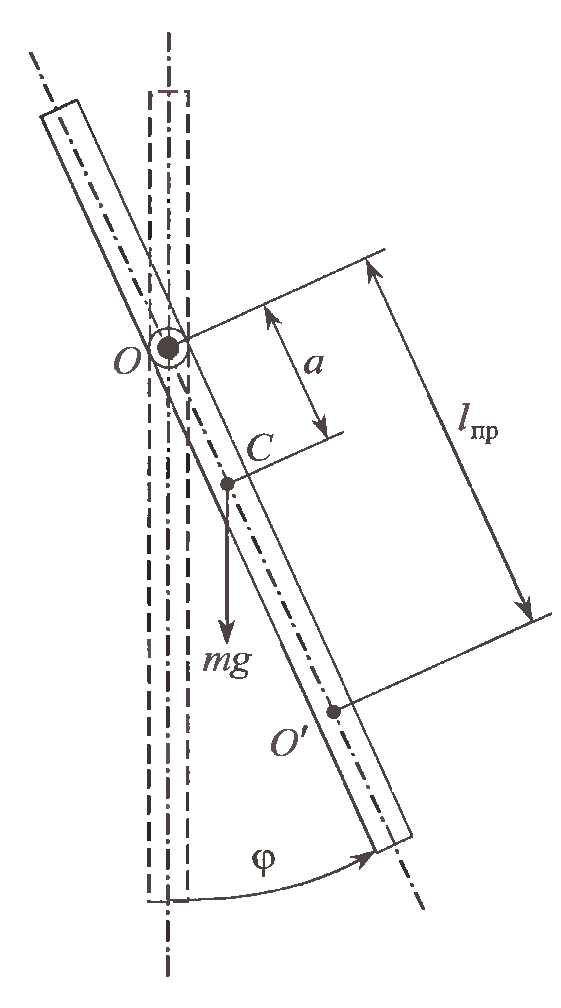
\includegraphics[width=1\linewidth]{ustanovka}
		\caption{Физический маятник}\label{risunok}
	\end{wrapfigure}
	
	\par В работе изучается динамика движения физического маятника.
	Физический маятник, используемый в работе, представляет собой однородный стальной стержень массы $m$, длина которого $l$ много больше ее диаметра. На стержне закрепляется опорная призма, острое ребро которой является осью качания маятника.
	
	Второй закон Ньютона определяет динамику движения тела точечной массы m. Импульс тела $P=mv$ изменяется во времени $t$ под действием силы $F$:
	\begin{equation}
		F = \frac{dP}{dt}
	\end{equation}
	Если рассмотреть точечную массу, которая движется по окружности радиуса $r$ с угловой скоростью $\omega$, тогда линейная скорость $v = \omega r$, то формулу для силы можно преобразовать:
	\begin{equation}
		Fr = \frac{dP}{dt}r
	\end{equation}
	\begin{equation}
		M=\frac{dP}{dt}r=\frac{dL}{dt}
	\end{equation}
	\noindent где $L = J\omega$, и $J = mr^2$. Величину $J$ называют \textit{моментом инерции}.
	\begin{equation}
		J = \sum_{i=1} m_i r_i^2
	\end{equation}
	\par Посчитаем момент инерции для данного нам стержня, при вращении вокруг препендикулярной стержню оси. Для этого разобьем стержень на отрезки $dr$ и $dm = m\cdot\frac{dr}{l}$ и возьмем интеграл:
	\begin{equation}
		J_c = \int_{-\frac{l}{2}}^{\frac{l}{2}}r^2dm = \int_{-\frac{l}{2}}^{\frac{l}{2}}\frac{mr^2}{l}dr = \frac{ml^2}{12} 
	\end{equation}
	
	
	Призму можно перемещать вдоль стержня, меняя таким образом расстояние $ OC $ от точки опоры маятника до его центра масс. Пусть это расстояние равно $ a $. Тогда по теореме Гюйгенса-Штейнера момент инерции маятника
	
	\begin{equation}
		J=\frac{ml^2}{12}+ma^2,
	\end{equation}
	
	\noindent где $ m $ -- масса маятника.
	
	
	Период колебаний получим из дифференциального уравнения: 
	$$-m g a \alpha = \frac{dL}{dt} = \frac{d(J\overset{.}{\alpha})}{dt} = J \overset{..}{\alpha} \Rightarrow \overset{..}{\alpha}+\frac{m g a}{J} \alpha = 0 $$
	$$  \overset{..}{\alpha}+\omega^2 \alpha = 0$$ 
	$$ \omega = \sqrt{\frac{m g a}{J}} \Rightarrow T =  \frac{2\pi}{\omega} = 2\pi \sqrt{\frac{J}{m g a} }$$
	
	
	\noindent После подстановки период колебаний, для стержня длиной $l$ подвешенного на расстоянии $a$ от центра, равен:
	
	\begin{equation}\label{time_a}
		T=2\pi\sqrt{\frac{a^2+\frac{l^2}{12}}{ag}}
	\end{equation}
	
	Таким образом, период малых колебаний не зависит ни от начальной фазы, ни от амплитуды колебаний.
	\medspace
	
	Период колебаний математического маятника определяется формулой
	\begin{equation}
		T_\text{м}=2\pi\sqrt{\frac{l}{g}},
	\end{equation}
	где $ l $ -- длина математического маятника. Поэтому величину
	\begin{equation}\label{prived}
		l_\text{пр}=a+\frac{l^2}{12a}
	\end{equation}
	называют приведённой длиной математического маятника. Поэтому точку $ O' $ (см. рис. \ref{risunok}), отстоящую от точки опоры на расстояние $ l_\text{пр} $, называют центром качания физического маятника. Точка опоры и центр качания маятника обратимы, т.е. при качании маятника вокруг  точки $ O' $ период будет таким же, как и при качании вокруг точки $ O $.
	
	\section {Экспериментальная установка}
	Тонкий стальной стержень, подвешенный на прикрепленной к стене консоли с помощью небольшой призмы, которая опирается на поверхность консоли острым основанием. Призму можно перемещать вдоль стержня, изменяя положение точки подвеса. Период колебаний измеряется с помощью секундомера, расстояния измеряются линейкой и штангенциркулем. Положение центра масс можно определить с помощью балансирования маятника на вспомогательной подставке.
	
	
	
	\subsection{Расчет поправок}
	Если быть честными, то для вычисления периода следует использовать формулу, учитывающую оба тела (и стержень, и призму):
	\begin{equation}
		T = 2\pi\sqrt{\frac{J_\text{ст} + J_\text{пр}}{m_\text{ст}ga_\text{ст}-m_\text{пр}ga_\text{пр}}}
	\end{equation}
	Однако призма мала по размеру и массе, поэтому поправка на момент инерции призмы в условиях опыта составляет не более 0,1\% $\Rightarrow$ ей можно пренебречь.
	
	Сравним теперь моменты сил, действующие на призму и стержень при $a = 10$ см:
	\begin{equation}
		\frac{M_\text{пр}}{M_\text{ст}} = \frac{m_\text{пр}ga_\text{пр}}{m_\text{ст}ga_\text{ст}} \approx 10^{-2}
	\end{equation}
	
	В данном случае поправка достигает 1\% $\Rightarrow$ ей пренебречь нельзя. Учесть влияние призмы можно -- исключив $a_\text{пр}$, изменяя положение центра сиситемы. Пусть $X$ -- расстояние от центра масс системы до точки подвеса, тогда:
	\begin{equation}
		X=\frac{m_\text{ст}a_\text{ст}-m_\text{пр}a_\text{пр}}{m_\text{ст} + m_\text{пр}}
	\end{equation}
	
	
	Исключая из двух уравнений $a_\text{пр}$, получаем:
	\begin{equation}\label{period}
		T = 2\pi \sqrt{\frac{\frac{l^2}{12}+a^2}{g\beta X}}
	\end{equation}	
	\noindent где $\beta= 1+\frac{m_\text{пр}}{m_\text{ст}}$.
	\section{Задание}
	\subsection{Оценка погрешностей измерительных приборов и $g$}
	\textbf{Секундомер:} $ \sigma_c = 0,01 \text{ с}$\\
	\textbf{Линейка:} $ \sigma_\text{лин} = 0,05 \text{ см}$\\\\
	Погрешность $g$ зависит от точности измерения длин и периода колебаний. Длины измеряли линейкой. Наименьшее измеренное расстояние 15 см, а наибольшее 100 см. Абсолютная погрешность линейки: $\sigma_\text{лин} = 0,05 \text{ см}$. Тогда относительная погрешность длин составляет порядка $\varepsilon_\text{max}\approx0,3\%$  ($\frac{0,05см}{15см}\times100\% = 0,3\%$).\\\\
	\textbf{Вывод:} используемые в работе инструменты позволяют вести измерения длин с точностью вплоть до 0,1\%. Для получения конечного результата с данной точностью период колебаний следует измерять с той же относительной погрешностью: не хуже, чем $\varepsilon_\text{max}\approx0,3\%$.
	\subsection{Длина стержня и множитель $\beta$}
	
	Длина стержня $l = \left(  100,0 \pm 0,05\right)$ см, масса стержня $m =\left(  868,4 \pm 0,1\right)$ г, масса призмы $m_\text{пр}=\left( 75,7 \pm 0,1\right)$ г. Формула для множителя $\beta$:
	\begin{equation}
		\beta=1+\frac{m_\text{пр}}{m}
	\end{equation}
	
	\noindent Рассчитаем множитель используя снятые массы: $\beta = 1+\frac{75,7}{868,4}\approx1,08717$. Погрешность  $\sigma_\text{$\beta$}$ будет рассчитывается по формуле:
	\begin{equation}
		\sigma_\text{$\beta$}=\beta\sqrt{\left(\frac{\sigma_\text{пр}}{m_\text{пр}}\right)^2+\left(\frac{\sigma}{m}\right)^2}
	\end{equation}
	\begin{equation}
		\sigma_\text{$\beta$}=1,08717\sqrt{\left(\frac{0,1}{75,7}\right)^2+\left(\frac{0,1}{868,4}\right)^2}\approx 1,44\cdot 10^{-3}
	\end{equation}
	\par Получаем, что $\beta = \left( 1,08717 \pm 0,00144\right)$ с учетом погрешности. В соответствии с правилами округления получаем, что $\beta$ следует округлять до четырех знаков после запятой: $\beta = \left( 1,0872 \pm 0,0014\right)$.
	
	\subsection{Центр масс стержня и конструкции}
	Центр масс стержня расположен на расстоянии $b = (50, 05 \pm 0,05) \text{ см}$ от одного из его концов. Острие призмы расположено на расстоянии $a = (20,00 \pm 0,05) \text{ см}$. 
	Сбалансировав маятник \emph{с призмой} на острие вспомогательной установки, измерим положение центра масс конструкции $x_\text{ц} = 27,3\text{ см}$. Определение точного положения центра масс усложняется тем, что достичь точного равновесия конструкции на установке почти невозможно, поэтому погрешность измерения увеличится: $x_\text{ц} = (27,3 \pm 0,1)\text{ см}$.
	
	\subsection{Предварительный опыт}
	Установим маятник на консоли и отклоним его на малый угол $\varphi_0 \approx 5^\circ$. Измерим время $n = 20$ полных колебаний и вычислим период колебаний $T = t/n$. Результаты измерений приведем в таблице \ref{tab1}.
	\begin{table}[H]
		\begin{center}
			\begin{tabular}{|c|c|c|c|c|}
				\hline
				№ & 1 & 2 & 3 & ср. \\
				\hline
				$t$, c & 30,54 & 30,56 & 30,55 & 30,55 \\ 
				\hline
				$T$, с & 1,527 & 1,528 & 1,528 & 1,528\\ 
				\hline
				$\Delta T$, c& 0,001 & 0,001 & 0,001 & 0,001 \\
				\hline
			\end{tabular}
		\end{center}
		\caption{Результаты измерения периода колебаний}
		\label{tab1}
	\end{table}
	
	Предварительное значение ускорения свободного падения посчитаем по формуле
	\begin{equation}\label{golos}
		g = \frac{4\pi^2 (\frac{l^2}{12} + a^2)}{T^2 \beta x_\text{ц}}
	\end{equation}
	\par Полученное значение равно $g = 9,74$ м/с$^2$. Отличие от табличного значения $g = 9,81$ м/с$^2$ составляет 
	\begin{equation}
		\alpha = \frac{9,81 - 9,74}{9,81}\times100\% = 0,71\%
	\end{equation}
	
	\par Так как случайная погрешность измерения времени пренебрежимо мала, полная погрешность измерения времени совпадает с приборной
		$$\sigma_\text{t} =  0,01\text{ c}$$
		$$\sigma_\text{T} = \frac{\sigma_\text{t}}{10} = 0,001\text{ c}$$
	\par Следовательно, с учетом погрешности период колебаний равен $T = 1,528 \pm 0,001$ с.
	
	\subsection{Измерение периода колебаний для различных значений $\text{a}$}
	
	Изменяем положение цилиндра, каждый раз измеряя его положение $a$ относительно центра и время 20 полных колебаний. Результаты приведены в таблице \ref{tab2}.
	
	
 			\begin{table}[htbp]
 				\centering
 				\caption{Результаты измерения периода колебаний для различных $\text{a}$}
 				\begin{tabular}{|r|r|r|r|r|}
 					\hline
 					$\text{№}$ & $\text{ц.м. цилиндра, cm}$ & $\text{Т за 20 периодов, s}$ &  $\text{Т, s}$ & $g,  \frac{m}{s^2}$ \\
 					\hline
 					1     & 73,9  & 32,44 & 1,622 & 9,82 \\
 					\hline
 					2     & 67,9  & 31,68 & 1,584 & 9,82 \\
 					\hline
 					3     & 61,9  & 30,99 & 1,550 & 9,81 \\
 					\hline
 					4     & 55,9  & 30,34 & 1,517 & 9,80 \\
 					\hline
 					5     & 49,9  & 29,74 & 1,487 & 9,81 \\
 					\hline
 					6     & 43,9  & 29,25 & 1,463 & 9,80 \\
 					\hline
 					7     & 37,9  & 28,84 & 1,442 & 9,81 \\
 					\hline
 					8     & 31,9  & 28,59 & 1,430 & 9,80 \\
 					\hline
 					9     & 25,9  & 28,47 & 1,424 & 9,80 \\
 					\hline
 					10    & 19,9  & 28,56 & 1,428 & 9,79 \\
 					\hline
 					11    & 13,9  & 28,85 & 1,443 & 9,79 \\
 					\hline
 					12    & 7,9   & 29,40 & 1,470 & 9,79 \\
 					\hline
 				\end{tabular}%
 				\label{tab2}
 			\end{table}%
 			
	
	\section{Обработка результатов измерений}
	\subsection{Усредненное значение $g$}
	Усредним значение $g = 9,81 \text{м/с}^2$. 
	
	По формуле \eqref{golos} Найдем систематическую погрешность $g$:
	\begin{equation}
		\sigma_g^\text{сист} = g\cdot \sqrt{\left(\frac{\sigma_{\frac{l^2}{12}+a^2}}{\frac{l^2}{12}+a^2}\right)^2+\left(\frac{\sigma_{T^2 \beta X}}{T^2\beta X}\right)^2}
	\end{equation}
	\begin{equation}
		\sigma_{\frac{l^2}{12}+a^2} = \sqrt{\left(\sigma_{l^2}^2+\sigma_{a^2}^2 \right)}
	\end{equation}
	\begin{equation}
		\sigma_g^\text{сист} =  g\cdot\sqrt{\frac{\left(\frac{2\sigma_l}{l} \right)^2 + \left(\frac{2\sigma_a}{a}\right)^2}{\left(\frac{l^2}{12}+a^2 \right)^2} + \left(\frac{2\sigma_T}{T}\right)^2+\left(\frac{\sigma_{\beta}}{\beta} \right)^2 + \left(\frac{\sigma_{X}}{X} \right)^2}		
	\end{equation}
	
	
	\begin{equation}
		\sigma_g^\text{сист} \approx 0,10 \frac{\text{м}}{c^2}
	\end{equation}
	
	
	Полную погрешность $g$ получим из $\sigma_g^\text{случ}$ и $\sigma_g^\text{сист}$:
	\begin{equation}
		\sigma_g^\text{полн} = \sqrt{(\sigma_g^\text{сист})^2+(\sigma_g^\text{случ})^2}\approx 0,10\frac{\text{м}}{c^2}	\end{equation}	
	где $\sigma_g^\text{случ} = 0,01 \frac{\text{м}}{c^2}   $.
	
	Тогда получаем: $g=\left( 9,81\pm 0,10\right) \frac{\text{м}}{c^2}$.
	
	\subsection{График $T(a)$}
	\begin{figure}[h!]
		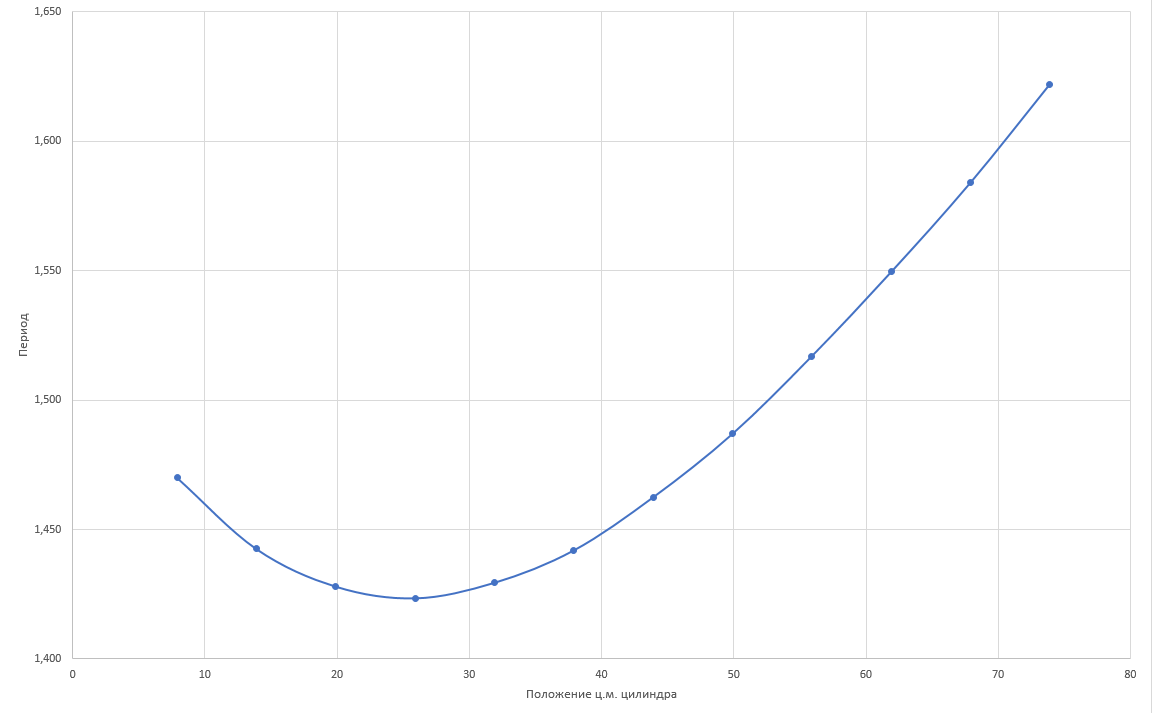
\includegraphics[scale=0.43]{graph}
		\caption{Зависимость $ T $ от $ a $}
		\label{graph}
	\end{figure}
	
	
	Минимум графика (Pисунок \ref{graph}) находится на $a_\textrm{min} \approx 27$ см, что сходится с рассчетом минимума по формуле \eqref{time_a}: $a_\textrm{формулы}\approx 27,3$ см
	\newpage
	\subsection{График зависимости $ T^2 x_\textrm{ц} $ от $C x_{\textrm{цил}}^2$ }

	
	\begin{table}[htbp]
		\centering
		
		\begin{tabular}{|r|r|r|r|r|}
			\hline
			$\textrm{№}$ & $x_c, cm$ & $T^2 x_c, m\cdot s^2$ & $C x_\textrm{цил}^2}, m^2$ & $g, \frac{m}{s^2}$ \\
			\hline
			1     & 38,92 & 1,0240 & 5,3771 & 9,82 \\
			\hline
			2     & 37,43 & 0,9390 & 4,5394 & 9,82 \\
			\hline
			3     & 35,93 & 0,8626 & 3,7726 & 9,81 \\
			\hline
			4     & 34,43 & 0,7924 & 3,0767 & 9,80 \\
			\hline
			5     & 32,94 & 0,7283 & 2,4517 & 9,81 \\
			\hline
			6     & 31,44 & 0,6725 & 1,8975 & 9,80 \\
			\hline
			7     & 29,94 & 0,6226 & 1,4143 & 9,81 \\
			\hline
			8     & 28,45 & 0,5813 & 1,0019 & 9,80 \\
			\hline
			9     & 26,95 & 0,5461 & 0,6605 & 9,80 \\
			\hline
			10    & 25,45 & 0,5191 & 0,3899 & 9,79 \\
			\hline
			11    & 23,96 & 0,4985 & 0,1902 & 9,79 \\
			\hline
			12    & 22,46 & 0,4854 & 0,0614 & 9,79 \\
			\hline
		\end{tabular}%
		\label{tab:addlabel}%
	\end{table}%

	
	Используя формулу для периода физического маятника \eqref{period} получаем следующее соотношение:
	
	\begin{equation}
		T^2x_\text{ц}\beta=\frac{4\pi^2}{g}a^2+\frac{\pi^2l^2}{3g}.
	\end{equation}
	Иначе говоря:
	$$T^2x_\text{ц}g=\frac{4\pi^2 m_\textrm{цил}}{M}a^2+\frac{\pi^2l^2 m_\textrm{ст}}{3M} \Rightarrow C = 4\pi^2 \frac{m_{\text{цил}}}{M}$$
	\begin{center}
		(g в таблице было рассчитано по этой формуле)
	\end{center}
	
	
	Отсюда можно сделать вывод о том, что $ T^2x_\text{ц}\beta $ линейно зависит от $ a^2 $, поэтому это зависимость можно представить в виде
	
	\begin{equation}
		T^2x_\text{ц}\beta=ka^2+b,
	\end{equation}
	где
	\begin{equation}\label{koef}
		k=\frac{4\pi^2}{g}  \text{ и }  b = \frac{\pi^2l^2}{3g}.
	\end{equation}
	С другой стороны $ T^2x_\text{ц} $ линейно зависит от $C x_{\textrm{цил}}^2$
	
	График зависимости $ T^2 x_\text{ц} $ от $C x_{\text{цил}}^2}$ представлен на рисунке \ref*{graph_file}.
	
	По графику определяем коэффициент наклона $k = 9,864$ - это и будет ускорение свободного падения.
	\begin{figure}[h!]
		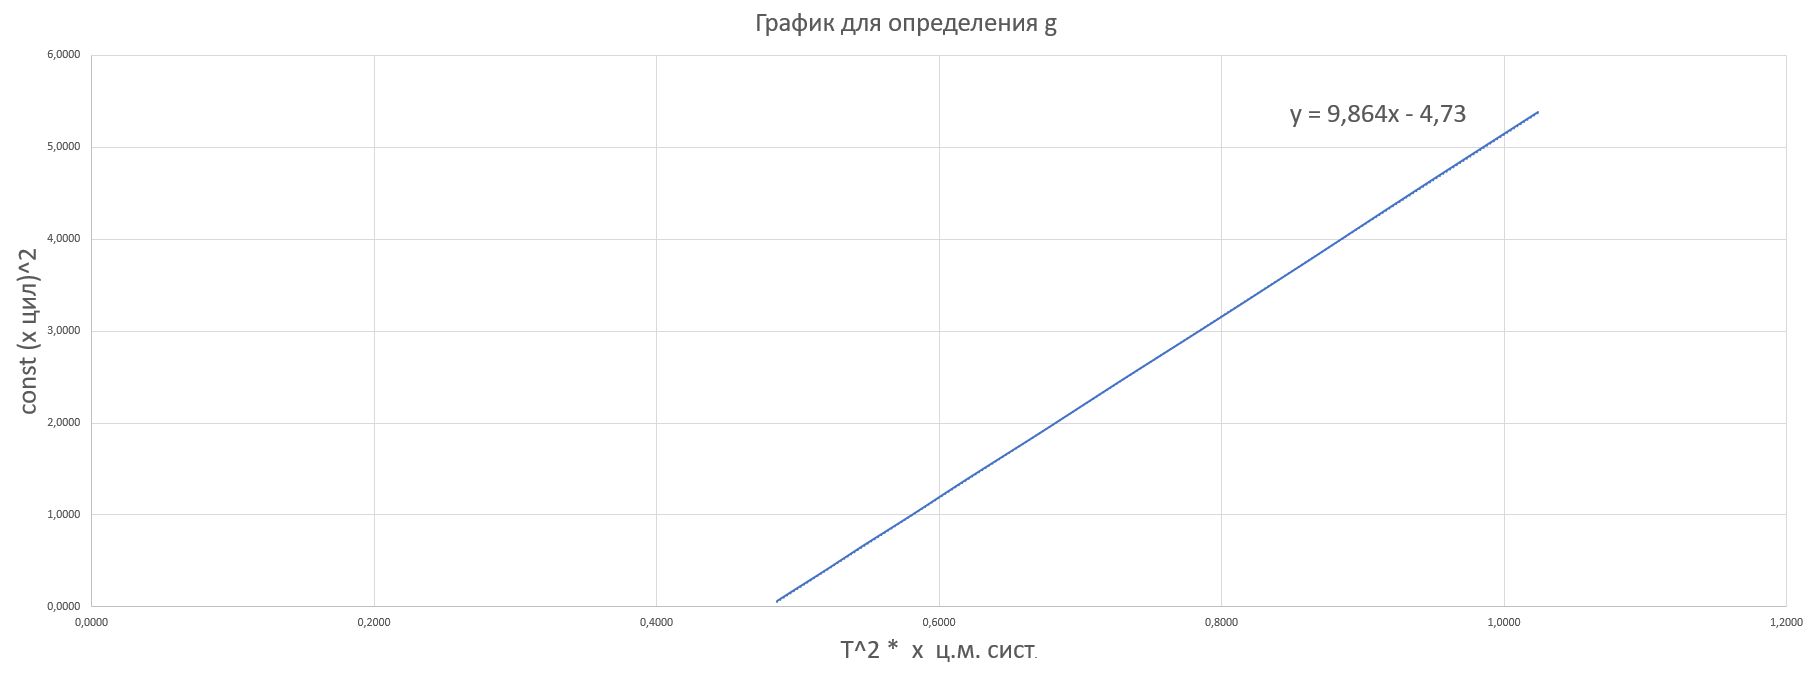
\includegraphics[scale=0.33]{graph_file}
		\caption{Зависимость $ T^2 x_\text{ц} $ от $C x_{\text{цил}}^2}$}
		\label{graph_file}
	\end{figure}
	\par
	Погрешность расчёта $ a^2 $ найдём по следующей формуле:
	
	\begin{equation}
		\varepsilon_{a^2}=2\varepsilon_a=2\frac{\sigma_a}{a}
	\end{equation}
	где $ \sigma_a = 0,1$ см.
	
	Погрешность вычисления $ T^2x_\text{ц}\beta $ можно найти по формуле:
	
	\begin{equation}
		\varepsilon_{T^2x_\text{ц}\beta} = \sqrt{\left( 2\cdot\frac{\sigma_T}{T} \right)^2 + \left(  \frac{\sigma_X}{X} \right)^2 + \left(\frac{\sigma_{\beta}}{\beta}\right)^2} \approx 0,01  ,
	\end{equation}
	
	Для вычисления коэффициентов $ k $ и $ b $ из \eqref{koef} воспользуемся методом наименьших квадратов:
	
	\begin{equation}
		k=\frac{\langle xy\rangle-\langle x\rangle \langle y\rangle}{\langle x^2\rangle - \langle x\rangle^2}\approx 0,0406\text{ }\frac{\text{с}^2}{\text{см}},
	\end{equation}
	
	\begin{equation}
		b=\langle y \rangle -k\langle x \rangle\approx 33,54\text{ }\text{см}\cdot\text{с}^2,
	\end{equation}
	где $ x=a^2 $, $ y=T^2x_\text{ц}\beta $.
	
	Случайные погрешности вычисления $ k $ и $ b $ можно найти по следующим формулам:
	
	\begin{equation}
		\sigma_k^\text{сл}=\frac{1}{\sqrt{N}}\sqrt{\frac{\langle y^2 \rangle - \langle y \rangle^2}{\langle x^2 \rangle - \langle x \rangle^2} - k^2  } \approx 2,08\cdot10^{-4} \text{ }\frac{\text{с}^2}{\text{см}},
	\end{equation}
	
	\begin{equation}
		\sigma_b^\text{сл}= \sigma_k^\text{сл} \sqrt{\langle x^2 \rangle - \langle x \rangle^2} \approx 0,11 \text{ }\text{см}\cdot\text{с}^2.
	\end{equation}
	
	Систематическая погрешность вычисления коэффициентов определяется следующим соотношением:
	
	\begin{equation}
		\sigma^\text{сист}_k = k\sqrt{\left( \varepsilon_{T^2X\beta} \right)^2 + \left( \varepsilon_{a^2} \right)^2 } \approx 4,5\cdot10^{-4} \text{ }\frac{\text{с}^2}{\text{см}},
	\end{equation}
	
	\begin{equation}
		\sigma^\text{сист}_b = b\sqrt{\left( \varepsilon_{T^2X\beta} \right)^2 + \left( \varepsilon_{a^2} \right)^2 } \approx  0,37 \text{ }\text{см}\cdot\text{с}^2.
	\end{equation}
	
	Тогда полную погрешность вычисления коэффициентов подсчитываем по следующей формуле:
	
	\begin{equation}
		\sigma_k = \sqrt{\left( \sigma_k^\text{сл} \right)^2 + \left( \sigma_k^\text{сист} \right)^2 } \approx 4,96\cdot 10^{-4} \text{ }\frac{\text{с}^2}{\text{см}},
	\end{equation}
	
	\begin{equation}
		\sigma_b = \sqrt{\left( \sigma_b^\text{сл} \right)^2 + \left( \sigma_b^\text{сист} \right)^2 } \approx 0,39 \text{ }\text{см}\cdot\text{с}^2.
	\end{equation}
	
	Таким образом, получаем:
	\begin{itemize}
		\item $ k = \left( 0,0406\pm 4,96\cdot10^{-4}\right)  \text{ }\frac{\text{с}^2}{\text{см}} $, $ \varepsilon_k = 1,22 \% $
		\item $ b = \left( 33,54\pm 0,39 \right)  \text{ }\text{см}\cdot\text{с}^2 $, $ \varepsilon_b = 1,16 \% $
	\end{itemize}
	
	Учитывая формулу \eqref{koef}, вычисляем $ g $ через угол наклона прямой:
	
	\begin{equation}
		g_k = \frac{4\pi^2}{k} \approx 9,723  \text{ }\frac{\text{м}}{\text{с}^2},
	\end{equation}
	
	\begin{equation}
		\sigma_{gk} = g\cdot\varepsilon_k \approx 0,088 \text{ }\frac{\text{м}}{\text{с}^2},
	\end{equation}
	
	
	
	Учитывая формулу \eqref{koef}, вычисляем $ g $ через пересечение с осью "y":
	
	\begin{equation}
		g_b = \frac{\pi^2l^2}{3b} \approx 9,809  \text{ }\frac{\text{м}}{\text{с}^2},
	\end{equation}
	
	\begin{equation}
		\sigma_{gb} = g\cdot\varepsilon_b \approx 0,114 \text{ }\frac{\text{м}}{\text{с}^2},
	\end{equation}
	
	
	
	В итоге имеем следующие результаты:
	
	\begin{itemize}
		
		\item \underline{$ g_k = \left( 9,723\pm 0,088\right) \frac{\text{м}}{\text{с}^2} $, $ \varepsilon_{gk} = 1,22\% $}
		
		\item \underline{$ g_b = \left( 9,809\pm 0,114\right) \frac{\text{м}}{\text{с}^2} $, $ \varepsilon_{gb} = 1,16\% $}
		
		\item \underline{$ g_{line}= \left( 9,864\pm 0,100\right) \frac{\text{м}}{\text{с}^2} $, $ \varepsilon_{g_{line}} \approx 1,01\% $}
		
		\item \underline{$ g_{anal}= \left( 9,80\pm 0,10\right) \frac{\text{м}}{\text{с}^2} $, $ \varepsilon_{g_{anal}} \approx 1,02\% $}
		
	\end{itemize}
	
	
	Исходя из полученных данных, пожно сказать, что все использованные методы определения $g$ дают довольно хороший результат, но особенно удивляет точность определения $g$ по свободному члену МНК. Так как случайная погрешность очень мала, основной вклад вносят погрешности приборов, поэтому погрешность можно увеличить за счет повышения точности используемого оборудования.
	
	
	\section{Вывод}
	Проделанный опыт подтверждает теорию для периода колебаний физического маятника. 
	
	В ходе работы мы получили следующие величины:

		\begin{itemize}
			
			\item $ g_k = \left( 9,723\pm 0,088\right) \frac{\text{м}}{\text{с}^2} $, $ \varepsilon_{gk} = 1,22\% $
			
			\item $ g_b = \left( 9,809\pm 0,114\right) \frac{\text{м}}{\text{с}^2} $, $ \varepsilon_{gb} = 1,16\% $
			
			\item $ g_{line}= \left( 9,864\pm 0,100\right) \frac{\text{м}}{\text{с}^2} $, $ \varepsilon_{g_{line}} \approx 1,01\% $
			
			\item $ g_{anal}= \left( 9,80\pm 0,10\right) \frac{\text{м}}{\text{с}^2} $, $ \varepsilon_{g_{anal}} \approx 1,02\% $
			
		\end{itemize}

	
	
	Точность полученных результатов можно повысить, если использовать более точные приборы. Погрешность вносит неточность определения расстояния от точки опоры до центра масс стержня, а также смещенный центр масс цилиндра. Последнюю погрешность можно нивелировать за счет использования двух цилиндров, расположенных симметрично, так чтобы их центр масс лежал на стержне.
	
	
	
	
	
	
\end{document}